\section{Retrieving Images in Clusters}
\label{sec_introduction}

\todo{introduce the introduction?}

\subsection{Problem Statement \& Motivation}
Many algorithms, e.g. for image categorization or content detection, require training data on which the relevant features can be learned. Obtaining such training data can be a quite troublesome task, especially when building a training set manually from scratch. If, for example, an algorithm shall be trained to identify and differentiate kinds of food, one would have to think of all possible kinds of food, search corresponding images and group them into homogenous groups. \\
Online photo communities like Flickr\footnote{https://www.flickr.com/} provide vast amounts of images, which are usually collaboratively tagged. These communities are therefore considered folksonomies\index{Folksonomy}, i.e. socially indexed collections.
Floksonomies can be good sources for training data, but several problems exist: First of all, annotations are often of poor quality, since anyone can tag anything without control mechanisms. Secondly, one can only search for one specific term, and will obtain images for all of the term's meanings, while the retrieval is limited to those images with the exact tag already. Furthermore, the images will be of a very large visual diversity, which is often not desired. \\

The above mentioned difficulties will be adressed by the tool presented in this work, whose main aim is to create homogeneous groups of semantically and visually similar pictures for a given topic in order to aid with the laborious assembly of training and test data sets. This is done based on the 1 million images of the MIRFLICKR-1M\footnote{http://press.liacs.nl/mirflickr/} file set. \\
When creating such a tool, one faces serveral challenges, like homonymy\index{Homonymy} of keywords (that is, the fact that one word can have multiple meanings), low quality of tags and other annotations, and the consideration of both semantic and visual information about a picture. \todo{further challenges?} 

\subsection{Clustered Tree Nodes Approach}
To achieve the stated goal, a Python web application was implemented, using SimpleCV\footnote{http://www.simplecv.org/} for visual image analysis and Flask\footnote{http://flask.pocoo.org/} for the frontend.\\
The tool provides ready-to-use semantically and visually homogeneous image clusters for a given topic, or searchterm. This is achieved by first spanning a tree of subordinate terms, retrieving related images by their keywords for each term, and then clustering the images by their predominant keywords as well as by colors and edge structure. These two major phases are illustrated in figure \ref{fig_overallprocess}.

\begin{figure}[h]
\centering
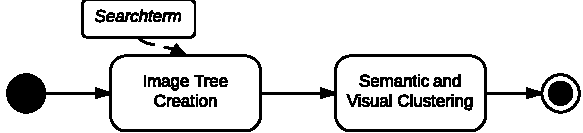
\includegraphics[]{images/search_process_highlevel.pdf}
\caption{The two main phases of our algorithm}
\label{fig_overallprocess}
\end{figure}

After giving an overview of Related Work in chapter 2, we will present how we analyze the image annotations and the user's search term to retrieve relevant images (chapter 3). The methods applied cluster these semantically and visually are described in chapter 4. Chapter 5 explains how we evaluate our approach, while the evaluation results will be discussed in chapter 6. At last, chapter 7 gives ideas for improvement and possible future work.
